% Options for packages loaded elsewhere
\PassOptionsToPackage{unicode}{hyperref}
\PassOptionsToPackage{hyphens}{url}
%
\documentclass[
]{article}
\usepackage{amsmath,amssymb}
\usepackage{lmodern}
\usepackage{iftex}
\ifPDFTeX
  \usepackage[T1]{fontenc}
  \usepackage[utf8]{inputenc}
  \usepackage{textcomp} % provide euro and other symbols
\else % if luatex or xetex
  \usepackage{unicode-math}
  \defaultfontfeatures{Scale=MatchLowercase}
  \defaultfontfeatures[\rmfamily]{Ligatures=TeX,Scale=1}
\fi
% Use upquote if available, for straight quotes in verbatim environments
\IfFileExists{upquote.sty}{\usepackage{upquote}}{}
\IfFileExists{microtype.sty}{% use microtype if available
  \usepackage[]{microtype}
  \UseMicrotypeSet[protrusion]{basicmath} % disable protrusion for tt fonts
}{}
\makeatletter
\@ifundefined{KOMAClassName}{% if non-KOMA class
  \IfFileExists{parskip.sty}{%
    \usepackage{parskip}
  }{% else
    \setlength{\parindent}{0pt}
    \setlength{\parskip}{6pt plus 2pt minus 1pt}}
}{% if KOMA class
  \KOMAoptions{parskip=half}}
\makeatother
\usepackage{xcolor}
\IfFileExists{xurl.sty}{\usepackage{xurl}}{} % add URL line breaks if available
\IfFileExists{bookmark.sty}{\usepackage{bookmark}}{\usepackage{hyperref}}
\hypersetup{
  pdftitle={hw3},
  pdfauthor={Yiting Zhang},
  hidelinks,
  pdfcreator={LaTeX via pandoc}}
\urlstyle{same} % disable monospaced font for URLs
\usepackage[margin=1in]{geometry}
\usepackage{color}
\usepackage{fancyvrb}
\newcommand{\VerbBar}{|}
\newcommand{\VERB}{\Verb[commandchars=\\\{\}]}
\DefineVerbatimEnvironment{Highlighting}{Verbatim}{commandchars=\\\{\}}
% Add ',fontsize=\small' for more characters per line
\usepackage{framed}
\definecolor{shadecolor}{RGB}{248,248,248}
\newenvironment{Shaded}{\begin{snugshade}}{\end{snugshade}}
\newcommand{\AlertTok}[1]{\textcolor[rgb]{0.94,0.16,0.16}{#1}}
\newcommand{\AnnotationTok}[1]{\textcolor[rgb]{0.56,0.35,0.01}{\textbf{\textit{#1}}}}
\newcommand{\AttributeTok}[1]{\textcolor[rgb]{0.77,0.63,0.00}{#1}}
\newcommand{\BaseNTok}[1]{\textcolor[rgb]{0.00,0.00,0.81}{#1}}
\newcommand{\BuiltInTok}[1]{#1}
\newcommand{\CharTok}[1]{\textcolor[rgb]{0.31,0.60,0.02}{#1}}
\newcommand{\CommentTok}[1]{\textcolor[rgb]{0.56,0.35,0.01}{\textit{#1}}}
\newcommand{\CommentVarTok}[1]{\textcolor[rgb]{0.56,0.35,0.01}{\textbf{\textit{#1}}}}
\newcommand{\ConstantTok}[1]{\textcolor[rgb]{0.00,0.00,0.00}{#1}}
\newcommand{\ControlFlowTok}[1]{\textcolor[rgb]{0.13,0.29,0.53}{\textbf{#1}}}
\newcommand{\DataTypeTok}[1]{\textcolor[rgb]{0.13,0.29,0.53}{#1}}
\newcommand{\DecValTok}[1]{\textcolor[rgb]{0.00,0.00,0.81}{#1}}
\newcommand{\DocumentationTok}[1]{\textcolor[rgb]{0.56,0.35,0.01}{\textbf{\textit{#1}}}}
\newcommand{\ErrorTok}[1]{\textcolor[rgb]{0.64,0.00,0.00}{\textbf{#1}}}
\newcommand{\ExtensionTok}[1]{#1}
\newcommand{\FloatTok}[1]{\textcolor[rgb]{0.00,0.00,0.81}{#1}}
\newcommand{\FunctionTok}[1]{\textcolor[rgb]{0.00,0.00,0.00}{#1}}
\newcommand{\ImportTok}[1]{#1}
\newcommand{\InformationTok}[1]{\textcolor[rgb]{0.56,0.35,0.01}{\textbf{\textit{#1}}}}
\newcommand{\KeywordTok}[1]{\textcolor[rgb]{0.13,0.29,0.53}{\textbf{#1}}}
\newcommand{\NormalTok}[1]{#1}
\newcommand{\OperatorTok}[1]{\textcolor[rgb]{0.81,0.36,0.00}{\textbf{#1}}}
\newcommand{\OtherTok}[1]{\textcolor[rgb]{0.56,0.35,0.01}{#1}}
\newcommand{\PreprocessorTok}[1]{\textcolor[rgb]{0.56,0.35,0.01}{\textit{#1}}}
\newcommand{\RegionMarkerTok}[1]{#1}
\newcommand{\SpecialCharTok}[1]{\textcolor[rgb]{0.00,0.00,0.00}{#1}}
\newcommand{\SpecialStringTok}[1]{\textcolor[rgb]{0.31,0.60,0.02}{#1}}
\newcommand{\StringTok}[1]{\textcolor[rgb]{0.31,0.60,0.02}{#1}}
\newcommand{\VariableTok}[1]{\textcolor[rgb]{0.00,0.00,0.00}{#1}}
\newcommand{\VerbatimStringTok}[1]{\textcolor[rgb]{0.31,0.60,0.02}{#1}}
\newcommand{\WarningTok}[1]{\textcolor[rgb]{0.56,0.35,0.01}{\textbf{\textit{#1}}}}
\usepackage{graphicx}
\makeatletter
\def\maxwidth{\ifdim\Gin@nat@width>\linewidth\linewidth\else\Gin@nat@width\fi}
\def\maxheight{\ifdim\Gin@nat@height>\textheight\textheight\else\Gin@nat@height\fi}
\makeatother
% Scale images if necessary, so that they will not overflow the page
% margins by default, and it is still possible to overwrite the defaults
% using explicit options in \includegraphics[width, height, ...]{}
\setkeys{Gin}{width=\maxwidth,height=\maxheight,keepaspectratio}
% Set default figure placement to htbp
\makeatletter
\def\fps@figure{htbp}
\makeatother
\setlength{\emergencystretch}{3em} % prevent overfull lines
\providecommand{\tightlist}{%
  \setlength{\itemsep}{0pt}\setlength{\parskip}{0pt}}
\setcounter{secnumdepth}{-\maxdimen} % remove section numbering
\ifLuaTeX
  \usepackage{selnolig}  % disable illegal ligatures
\fi

\title{hw3}
\author{Yiting Zhang}
\date{2022-04-20}

\begin{document}
\maketitle

\begin{Shaded}
\begin{Highlighting}[]
\NormalTok{titanic }\OtherTok{\textless{}{-}} \FunctionTok{read.csv}\NormalTok{(}\AttributeTok{file=}\StringTok{\textquotesingle{}titanic.csv\textquotesingle{}}\NormalTok{)}
\NormalTok{titanic}\SpecialCharTok{$}\NormalTok{survived }\OtherTok{\textless{}{-}} \FunctionTok{factor}\NormalTok{(titanic}\SpecialCharTok{$}\NormalTok{survived, }\AttributeTok{levels=}\FunctionTok{c}\NormalTok{ (}\StringTok{\textquotesingle{}Yes\textquotesingle{}}\NormalTok{,}\StringTok{\textquotesingle{}No\textquotesingle{}}\NormalTok{)) }
\NormalTok{titanic}\OtherTok{\textless{}{-}}\NormalTok{titanic}\SpecialCharTok{\%\textgreater{}\%}\FunctionTok{mutate}\NormalTok{(titanic}\SpecialCharTok{$}\NormalTok{survived)}\SpecialCharTok{\%\textgreater{}\%}\FunctionTok{mutate}\NormalTok{(}\AttributeTok{pclass=}\FunctionTok{factor}\NormalTok{(titanic}\SpecialCharTok{$}\NormalTok{pclass))}
\CommentTok{\#levels(titanic$survived)}
\CommentTok{\#head(titanic)}
\end{Highlighting}
\end{Shaded}

\hypertarget{question-1}{%
\subsubsection{Question 1}\label{question-1}}

\begin{Shaded}
\begin{Highlighting}[]
\CommentTok{\# Stratified Sampling}
\FunctionTok{set.seed}\NormalTok{(}\DecValTok{3435}\NormalTok{)}
\NormalTok{titanic\_split }\OtherTok{\textless{}{-}} \FunctionTok{initial\_split}\NormalTok{(titanic, }\AttributeTok{strata =}\NormalTok{ survived, }\AttributeTok{prop =} \FloatTok{0.8}\NormalTok{)}
\NormalTok{titanic\_split}
\end{Highlighting}
\end{Shaded}

\begin{verbatim}
## <Analysis/Assess/Total>
## <712/179/891>
\end{verbatim}

\begin{Shaded}
\begin{Highlighting}[]
\NormalTok{titanic\_train }\OtherTok{\textless{}{-}} \FunctionTok{training}\NormalTok{(titanic\_split)}
\NormalTok{titanic\_test }\OtherTok{\textless{}{-}} \FunctionTok{testing}\NormalTok{(titanic\_split)}

\NormalTok{data}\OtherTok{\textless{}{-}}\FunctionTok{dim}\NormalTok{(titanic)[}\DecValTok{1}\NormalTok{]}
\NormalTok{train}\OtherTok{\textless{}{-}}\FunctionTok{dim}\NormalTok{(titanic\_train)[}\DecValTok{1}\NormalTok{]}
\NormalTok{test}\OtherTok{\textless{}{-}}\FunctionTok{dim}\NormalTok{(titanic\_test)[}\DecValTok{1}\NormalTok{]}
\NormalTok{train}\SpecialCharTok{/}\NormalTok{data}
\end{Highlighting}
\end{Shaded}

\begin{verbatim}
## [1] 0.7991021
\end{verbatim}

\begin{Shaded}
\begin{Highlighting}[]
\NormalTok{test}\SpecialCharTok{/}\NormalTok{data}
\end{Highlighting}
\end{Shaded}

\begin{verbatim}
## [1] 0.2008979
\end{verbatim}

We can verify that the training and testing data sets have the
appropriate number of observations by calculating the ratio above.

In both the testing and training data, stratified sampling will retain
the real ratio of Survived,avoiding sampling error in which one dataset
has more observations where Survived is Yes than the other dataset.

\begin{Shaded}
\begin{Highlighting}[]
\FunctionTok{sum}\NormalTok{ (}\FunctionTok{is.na}\NormalTok{(titanic\_train))}
\end{Highlighting}
\end{Shaded}

\begin{verbatim}
## [1] 701
\end{verbatim}

There are 701 missing data in our titanic training dataset. This will
influence our model. But overall, the stratified sampling method is a
good idea. It enables us to collect a representative sample of the full
observation under investigation.

\hypertarget{question-2}{%
\subsubsection{Question 2}\label{question-2}}

\begin{Shaded}
\begin{Highlighting}[]
\CommentTok{\# Explore Distribution}
\NormalTok{titanic\_train }\SpecialCharTok{\%\textgreater{}\%} \FunctionTok{ggplot}\NormalTok{(}\FunctionTok{aes}\NormalTok{(}\AttributeTok{x=}\NormalTok{survived)) }\SpecialCharTok{+} \FunctionTok{geom\_bar}\NormalTok{()}
\end{Highlighting}
\end{Shaded}

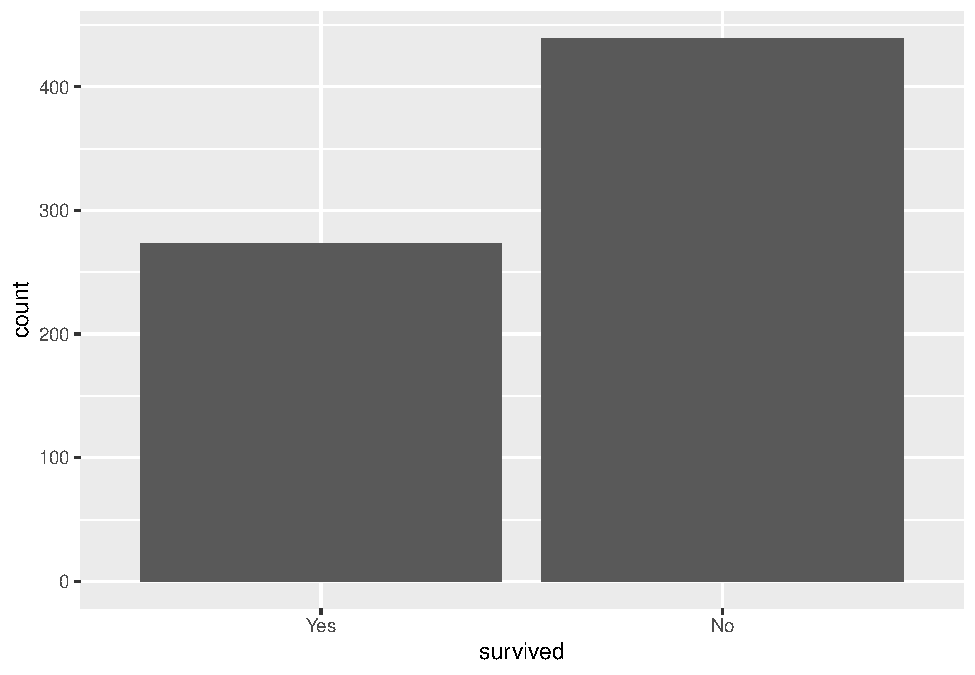
\includegraphics{hw3_files/figure-latex/unnamed-chunk-5-1.pdf}

We can observe from the plot that about over 450 the passengers in the
training dataset did not survive while only approximately 250 passengers
survived.

\hypertarget{question-3}{%
\subsubsection{Question 3}\label{question-3}}

\begin{Shaded}
\begin{Highlighting}[]
\CommentTok{\# Visualization}
\NormalTok{cor\_titanic }\OtherTok{\textless{}{-}}\NormalTok{ titanic\_train }\SpecialCharTok{\%\textgreater{}\%}
  \FunctionTok{select}\NormalTok{(}\FunctionTok{where}\NormalTok{(is.numeric)) }\SpecialCharTok{\%\textgreater{}\%}
  \FunctionTok{correlate}\NormalTok{()}
\FunctionTok{rplot}\NormalTok{(cor\_titanic)}
\end{Highlighting}
\end{Shaded}

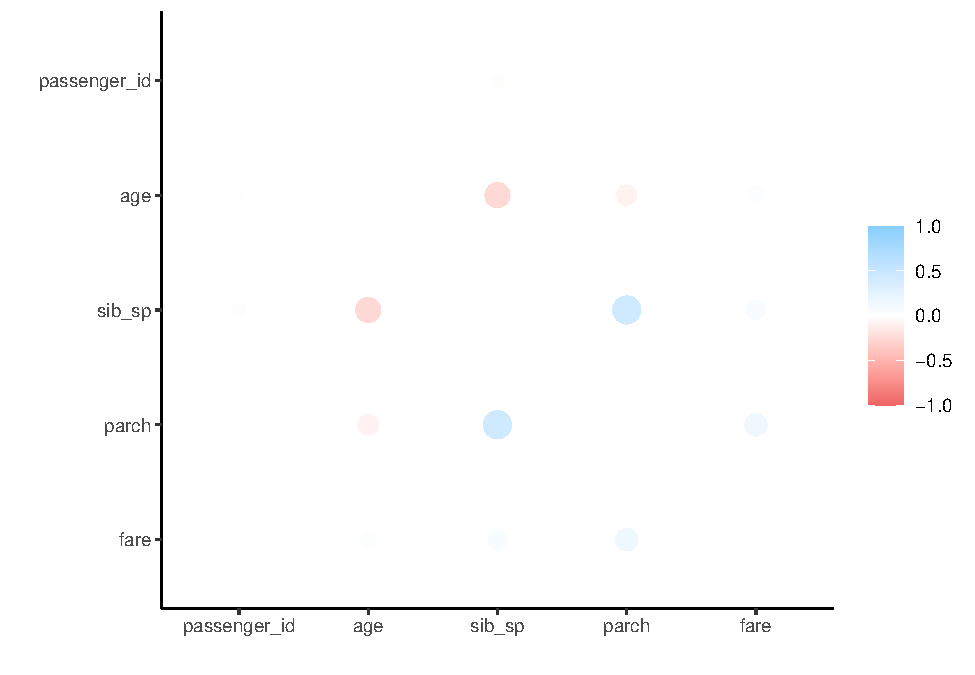
\includegraphics{hw3_files/figure-latex/unnamed-chunk-6-1.pdf}

\begin{Shaded}
\begin{Highlighting}[]
\NormalTok{cor\_titanic }\SpecialCharTok{\%\textgreater{}\%}
  \FunctionTok{stretch}\NormalTok{() }\SpecialCharTok{\%\textgreater{}\%}
  \FunctionTok{ggplot}\NormalTok{(}\FunctionTok{aes}\NormalTok{(x, y, }\AttributeTok{fill =}\NormalTok{ r)) }\SpecialCharTok{+}
  \FunctionTok{geom\_tile}\NormalTok{() }\SpecialCharTok{+}
  \FunctionTok{geom\_text}\NormalTok{(}\FunctionTok{aes}\NormalTok{(}\AttributeTok{label =} \FunctionTok{as.character}\NormalTok{(}\FunctionTok{fashion}\NormalTok{(r))))}
\end{Highlighting}
\end{Shaded}

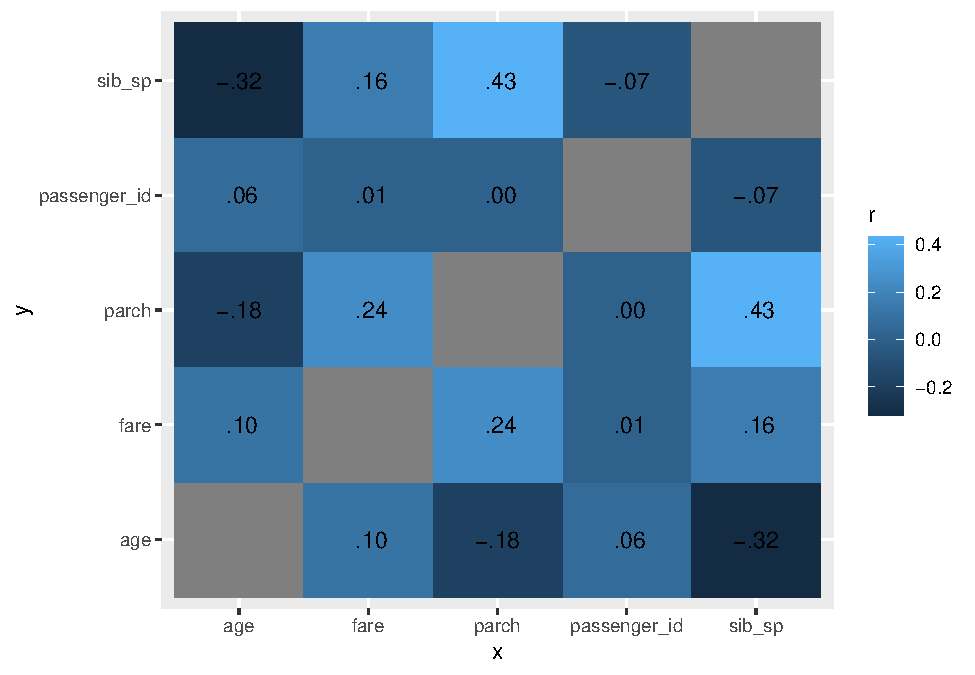
\includegraphics{hw3_files/figure-latex/unnamed-chunk-7-1.pdf} Number of
parents/children on board and number of siblings/spouses on board are
positively correlated. Number of parents/children on board and fare are
slightly positively correlated. Age and number of siblings/spouses on
board are negatively correlated. Number of parents/children and age are
negatively correlated.Passenger ID almost have no correlation with any
other predictors.

\hypertarget{question-4}{%
\subsubsection{Question 4}\label{question-4}}

\begin{Shaded}
\begin{Highlighting}[]
\CommentTok{\# Recipe}
\NormalTok{titanic\_recipe }\OtherTok{\textless{}{-}} \FunctionTok{recipe}\NormalTok{(survived }\SpecialCharTok{\textasciitilde{}}\NormalTok{ pclass }\SpecialCharTok{+}\NormalTok{ sex }\SpecialCharTok{+}\NormalTok{ age }\SpecialCharTok{+}\NormalTok{ sib\_sp }\SpecialCharTok{+}\NormalTok{ parch }\SpecialCharTok{+}\NormalTok{ fare,}
                         \AttributeTok{data =}\NormalTok{ titanic\_train) }\SpecialCharTok{\%\textgreater{}\%}
  \FunctionTok{step\_impute\_linear}\NormalTok{(age) }\SpecialCharTok{\%\textgreater{}\%}
  \FunctionTok{step\_dummy}\NormalTok{(}\FunctionTok{all\_nominal\_predictors}\NormalTok{()) }\SpecialCharTok{\%\textgreater{}\%}
  \FunctionTok{step\_interact}\NormalTok{(}\AttributeTok{terms =} \SpecialCharTok{\textasciitilde{}} \FunctionTok{starts\_with}\NormalTok{(}\StringTok{"sex"}\NormalTok{)}\SpecialCharTok{:}\NormalTok{fare) }\SpecialCharTok{\%\textgreater{}\%}
  \FunctionTok{step\_interact}\NormalTok{(}\AttributeTok{terms =} \SpecialCharTok{\textasciitilde{}}\NormalTok{ age}\SpecialCharTok{:}\NormalTok{fare)}
\end{Highlighting}
\end{Shaded}

\hypertarget{question-5}{%
\subsubsection{Question 5}\label{question-5}}

\begin{Shaded}
\begin{Highlighting}[]
\CommentTok{\# Specify an Engine}
\NormalTok{log\_reg }\OtherTok{\textless{}{-}} \FunctionTok{logistic\_reg}\NormalTok{() }\SpecialCharTok{\%\textgreater{}\%}
  \FunctionTok{set\_engine}\NormalTok{(}\StringTok{"glm"}\NormalTok{) }\SpecialCharTok{\%\textgreater{}\%}
  \FunctionTok{set\_mode}\NormalTok{(}\StringTok{"classification"}\NormalTok{)}
\CommentTok{\# Workflow}
\NormalTok{log\_wkflow }\OtherTok{\textless{}{-}} \FunctionTok{workflow}\NormalTok{() }\SpecialCharTok{\%\textgreater{}\%}
  \FunctionTok{add\_model}\NormalTok{(log\_reg) }\SpecialCharTok{\%\textgreater{}\%}
  \FunctionTok{add\_recipe}\NormalTok{(titanic\_recipe)}

\NormalTok{log\_fit }\OtherTok{\textless{}{-}} \FunctionTok{fit}\NormalTok{(log\_wkflow, titanic\_train)}

\CommentTok{\# Model Results}
\NormalTok{log\_fit }\SpecialCharTok{\%\textgreater{}\%}
  \FunctionTok{tidy}\NormalTok{()}
\end{Highlighting}
\end{Shaded}

\begin{verbatim}
## # A tibble: 10 x 5
##    term             estimate std.error statistic  p.value
##    <chr>               <dbl>     <dbl>     <dbl>    <dbl>
##  1 (Intercept)     -4.34      0.651       -6.66  2.72e-11
##  2 age              0.0606    0.0128       4.75  1.99e- 6
##  3 sib_sp           0.436     0.129        3.37  7.57e- 4
##  4 parch            0.280     0.151        1.85  6.40e- 2
##  5 fare            -0.00639   0.0109      -0.587 5.57e- 1
##  6 pclass_X2        1.16      0.343        3.39  6.92e- 4
##  7 pclass_X3        2.33      0.361        6.45  1.15e-10
##  8 sex_male         2.37      0.297        8.00  1.29e-15
##  9 sex_male_x_fare  0.0136    0.00859      1.59  1.13e- 1
## 10 age_x_fare      -0.000281  0.000190    -1.48  1.39e- 1
\end{verbatim}

\hypertarget{question-6}{%
\subsubsection{Question 6}\label{question-6}}

\begin{Shaded}
\begin{Highlighting}[]
\CommentTok{\# LDA}
\NormalTok{lda\_mod }\OtherTok{\textless{}{-}} \FunctionTok{discrim\_linear}\NormalTok{() }\SpecialCharTok{\%\textgreater{}\%}
  \FunctionTok{set\_mode}\NormalTok{(}\StringTok{"classification"}\NormalTok{) }\SpecialCharTok{\%\textgreater{}\%}
  \FunctionTok{set\_engine}\NormalTok{(}\StringTok{"MASS"}\NormalTok{)}

\NormalTok{lda\_wkflow }\OtherTok{\textless{}{-}} \FunctionTok{workflow}\NormalTok{() }\SpecialCharTok{\%\textgreater{}\%}
  \FunctionTok{add\_model}\NormalTok{(lda\_mod) }\SpecialCharTok{\%\textgreater{}\%}
  \FunctionTok{add\_recipe}\NormalTok{(titanic\_recipe)}

\NormalTok{lda\_fit }\OtherTok{\textless{}{-}} \FunctionTok{fit}\NormalTok{(lda\_wkflow, titanic\_train)}
\end{Highlighting}
\end{Shaded}

\hypertarget{question-7}{%
\subsubsection{Question 7}\label{question-7}}

\begin{Shaded}
\begin{Highlighting}[]
\CommentTok{\# QDA}
\NormalTok{qda\_mod }\OtherTok{\textless{}{-}} \FunctionTok{discrim\_quad}\NormalTok{() }\SpecialCharTok{\%\textgreater{}\%}
  \FunctionTok{set\_mode}\NormalTok{(}\StringTok{"classification"}\NormalTok{) }\SpecialCharTok{\%\textgreater{}\%}
  \FunctionTok{set\_engine}\NormalTok{(}\StringTok{"MASS"}\NormalTok{)}

\NormalTok{qda\_wkflow }\OtherTok{\textless{}{-}} \FunctionTok{workflow}\NormalTok{() }\SpecialCharTok{\%\textgreater{}\%}
  \FunctionTok{add\_model}\NormalTok{(qda\_mod) }\SpecialCharTok{\%\textgreater{}\%}
  \FunctionTok{add\_recipe}\NormalTok{(titanic\_recipe)}

\NormalTok{qda\_fit }\OtherTok{\textless{}{-}} \FunctionTok{fit}\NormalTok{(qda\_wkflow, titanic\_train)}
\end{Highlighting}
\end{Shaded}

\hypertarget{question-8}{%
\subsubsection{Question 8}\label{question-8}}

\begin{Shaded}
\begin{Highlighting}[]
\CommentTok{\# Naive Bayes}
\NormalTok{nb\_mod }\OtherTok{\textless{}{-}} \FunctionTok{naive\_Bayes}\NormalTok{() }\SpecialCharTok{\%\textgreater{}\%}
  \FunctionTok{set\_mode}\NormalTok{(}\StringTok{"classification"}\NormalTok{) }\SpecialCharTok{\%\textgreater{}\%}
  \FunctionTok{set\_engine}\NormalTok{(}\StringTok{"klaR"}\NormalTok{) }\SpecialCharTok{\%\textgreater{}\%}
  \FunctionTok{set\_args}\NormalTok{(}\AttributeTok{usekernel =} \ConstantTok{FALSE}\NormalTok{)}

\NormalTok{nb\_wkflow }\OtherTok{\textless{}{-}} \FunctionTok{workflow}\NormalTok{() }\SpecialCharTok{\%\textgreater{}\%}
  \FunctionTok{add\_model}\NormalTok{(nb\_mod) }\SpecialCharTok{\%\textgreater{}\%}
  \FunctionTok{add\_recipe}\NormalTok{(titanic\_recipe)}

\NormalTok{nb\_fit }\OtherTok{\textless{}{-}} \FunctionTok{fit}\NormalTok{(nb\_wkflow, titanic\_train)}
\end{Highlighting}
\end{Shaded}

\hypertarget{question-9}{%
\subsubsection{Question 9}\label{question-9}}

\begin{Shaded}
\begin{Highlighting}[]
\NormalTok{log\_predict}\OtherTok{\textless{}{-}}\FunctionTok{predict}\NormalTok{(log\_fit, }\AttributeTok{new\_data =}\NormalTok{ titanic\_train, }\AttributeTok{type =} \StringTok{"prob"}\NormalTok{)}

\NormalTok{log\_reg\_acc }\OtherTok{\textless{}{-}} \FunctionTok{augment}\NormalTok{(log\_fit, }\AttributeTok{new\_data =}\NormalTok{ titanic\_train) }\SpecialCharTok{\%\textgreater{}\%}
  \FunctionTok{accuracy}\NormalTok{(}\AttributeTok{truth =}\NormalTok{ survived, }\AttributeTok{estimate =}\NormalTok{ .pred\_class)}
\NormalTok{log\_reg\_acc}
\end{Highlighting}
\end{Shaded}

\begin{verbatim}
## # A tibble: 1 x 3
##   .metric  .estimator .estimate
##   <chr>    <chr>          <dbl>
## 1 accuracy binary         0.816
\end{verbatim}

\begin{Shaded}
\begin{Highlighting}[]
\NormalTok{lda\_predict}\OtherTok{\textless{}{-}}\FunctionTok{predict}\NormalTok{(lda\_fit, }\AttributeTok{new\_data =}\NormalTok{ titanic\_train, }\AttributeTok{type =} \StringTok{"prob"}\NormalTok{)}

\NormalTok{lda\_acc }\OtherTok{\textless{}{-}} \FunctionTok{augment}\NormalTok{(lda\_fit, }\AttributeTok{new\_data =}\NormalTok{ titanic\_train) }\SpecialCharTok{\%\textgreater{}\%}
  \FunctionTok{accuracy}\NormalTok{(}\AttributeTok{truth =}\NormalTok{ survived, }\AttributeTok{estimate =}\NormalTok{ .pred\_class)}
\NormalTok{lda\_acc}
\end{Highlighting}
\end{Shaded}

\begin{verbatim}
## # A tibble: 1 x 3
##   .metric  .estimator .estimate
##   <chr>    <chr>          <dbl>
## 1 accuracy binary         0.806
\end{verbatim}

\begin{Shaded}
\begin{Highlighting}[]
\NormalTok{qda\_predict}\OtherTok{\textless{}{-}}\FunctionTok{predict}\NormalTok{(qda\_fit, }\AttributeTok{new\_data =}\NormalTok{ titanic\_train, }\AttributeTok{type =} \StringTok{"prob"}\NormalTok{)}

\NormalTok{qda\_acc }\OtherTok{\textless{}{-}} \FunctionTok{augment}\NormalTok{(qda\_fit, }\AttributeTok{new\_data =}\NormalTok{ titanic\_train) }\SpecialCharTok{\%\textgreater{}\%}
  \FunctionTok{accuracy}\NormalTok{(}\AttributeTok{truth =}\NormalTok{ survived, }\AttributeTok{estimate =}\NormalTok{ .pred\_class)}
\NormalTok{qda\_acc}
\end{Highlighting}
\end{Shaded}

\begin{verbatim}
## # A tibble: 1 x 3
##   .metric  .estimator .estimate
##   <chr>    <chr>          <dbl>
## 1 accuracy binary         0.787
\end{verbatim}

\begin{Shaded}
\begin{Highlighting}[]
\NormalTok{nb\_predict}\OtherTok{\textless{}{-}}\FunctionTok{predict}\NormalTok{(nb\_fit, }\AttributeTok{new\_data =}\NormalTok{ titanic\_train, }\AttributeTok{type =} \StringTok{"prob"}\NormalTok{)}

\NormalTok{nb\_acc }\OtherTok{\textless{}{-}} \FunctionTok{augment}\NormalTok{(nb\_fit, }\AttributeTok{new\_data =}\NormalTok{ titanic\_train) }\SpecialCharTok{\%\textgreater{}\%}
  \FunctionTok{accuracy}\NormalTok{(}\AttributeTok{truth =}\NormalTok{ survived, }\AttributeTok{estimate =}\NormalTok{ .pred\_class)}
\NormalTok{nb\_acc}
\end{Highlighting}
\end{Shaded}

\begin{verbatim}
## # A tibble: 1 x 3
##   .metric  .estimator .estimate
##   <chr>    <chr>          <dbl>
## 1 accuracy binary         0.778
\end{verbatim}

\begin{Shaded}
\begin{Highlighting}[]
\NormalTok{pred\_df }\OtherTok{\textless{}{-}} \FunctionTok{bind\_cols}\NormalTok{(log\_predict, lda\_predict, qda\_predict, nb\_predict, titanic\_train}\SpecialCharTok{$}\NormalTok{survived)}
\NormalTok{names }\OtherTok{\textless{}{-}} \FunctionTok{c}\NormalTok{(}\StringTok{"Logistic Regression"}\NormalTok{, }\StringTok{"Linear Discriminant Analysis"}\NormalTok{, }\StringTok{"Quadratic Discriminant Analysis"}\NormalTok{, }\StringTok{"Naive Bayes"}\NormalTok{, }\StringTok{"Actual Data"}\NormalTok{)}
\FunctionTok{colnames}\NormalTok{(pred\_df)}\SpecialCharTok{\%\textgreater{}\%}\NormalTok{names}
\end{Highlighting}
\end{Shaded}

\begin{verbatim}
## NULL
\end{verbatim}

\begin{Shaded}
\begin{Highlighting}[]
\NormalTok{pred\_df}
\end{Highlighting}
\end{Shaded}

\begin{verbatim}
## # A tibble: 712 x 9
##    .pred_Yes...1 .pred_No...2 .pred_Yes...3 .pred_No...4 .pred_Yes...5
##            <dbl>        <dbl>         <dbl>        <dbl>         <dbl>
##  1        0.106         0.894       0.0636         0.936  0.00581     
##  2        0.0786        0.921       0.0453         0.955  0.00442     
##  3        0.290         0.710       0.237          0.763  0.0608      
##  4        0.0990        0.901       0.0679         0.932  0.0000344   
##  5        0.0116        0.988       0.00692        0.993  0.0000000163
##  6        0.776         0.224       0.839          0.161  0.599       
##  7        0.0631        0.937       0.0473         0.953  0.000000119 
##  8        0.492         0.508       0.593          0.407  0.265       
##  9        0.222         0.778       0.156          0.844  0.00958     
## 10        0.530         0.470       0.645          0.355  0.000674    
## # ... with 702 more rows, and 4 more variables: .pred_No...6 <dbl>,
## #   .pred_Yes...7 <dbl>, .pred_No...8 <dbl>, ...9 <fct>
\end{verbatim}

\begin{Shaded}
\begin{Highlighting}[]
\CommentTok{\# Comparing Model Performance}
\NormalTok{accuracies }\OtherTok{\textless{}{-}} \FunctionTok{c}\NormalTok{(log\_reg\_acc}\SpecialCharTok{$}\NormalTok{.estimate, lda\_acc}\SpecialCharTok{$}\NormalTok{.estimate,}
\NormalTok{                nb\_acc}\SpecialCharTok{$}\NormalTok{.estimate, qda\_acc}\SpecialCharTok{$}\NormalTok{.estimate)}
\NormalTok{models }\OtherTok{\textless{}{-}} \FunctionTok{c}\NormalTok{(}\StringTok{"Logistic Regression"}\NormalTok{, }\StringTok{"LDA"}\NormalTok{, }\StringTok{"Naive Bayes"}\NormalTok{, }\StringTok{"QDA"}\NormalTok{)}
\NormalTok{results }\OtherTok{\textless{}{-}} \FunctionTok{tibble}\NormalTok{(}\AttributeTok{accuracies =}\NormalTok{ accuracies, }\AttributeTok{models =}\NormalTok{ models)}
\NormalTok{results }\SpecialCharTok{\%\textgreater{}\%}
  \FunctionTok{arrange}\NormalTok{(}\SpecialCharTok{{-}}\NormalTok{accuracies)}
\end{Highlighting}
\end{Shaded}

\begin{verbatim}
## # A tibble: 4 x 2
##   accuracies models             
##        <dbl> <chr>              
## 1      0.816 Logistic Regression
## 2      0.806 LDA                
## 3      0.787 QDA                
## 4      0.778 Naive Bayes
\end{verbatim}

Therefore, by comparing the four models, we find that logistic
regression model got the highest accuracy on the training data.

\hypertarget{question-10}{%
\subsubsection{Question 10}\label{question-10}}

\begin{Shaded}
\begin{Highlighting}[]
\CommentTok{\# Fitting to Testing Data}
\FunctionTok{predict}\NormalTok{(log\_fit, }\AttributeTok{new\_data =}\NormalTok{ titanic\_test, }\AttributeTok{type =} \StringTok{"prob"}\NormalTok{)}
\end{Highlighting}
\end{Shaded}

\begin{verbatim}
## # A tibble: 179 x 2
##    .pred_Yes .pred_No
##        <dbl>    <dbl>
##  1    0.110    0.890 
##  2    0.493    0.507 
##  3    0.806    0.194 
##  4    0.170    0.830 
##  5    0.169    0.831 
##  6    0.0440   0.956 
##  7    0.162    0.838 
##  8    0.563    0.437 
##  9    0.909    0.0913
## 10    0.722    0.278 
## # ... with 169 more rows
\end{verbatim}

\begin{Shaded}
\begin{Highlighting}[]
\CommentTok{\# Check testing accuracy}
\NormalTok{multi\_metric }\OtherTok{\textless{}{-}} \FunctionTok{metric\_set}\NormalTok{(accuracy, sensitivity, specificity)}

\FunctionTok{augment}\NormalTok{(log\_fit, }\AttributeTok{new\_data =}\NormalTok{ titanic\_train) }\SpecialCharTok{\%\textgreater{}\%}
  \FunctionTok{multi\_metric}\NormalTok{(}\AttributeTok{truth =}\NormalTok{ survived, }\AttributeTok{estimate =}\NormalTok{ .pred\_class)}
\end{Highlighting}
\end{Shaded}

\begin{verbatim}
## # A tibble: 3 x 3
##   .metric     .estimator .estimate
##   <chr>       <chr>          <dbl>
## 1 accuracy    binary         0.816
## 2 sensitivity binary         0.692
## 3 specificity binary         0.893
\end{verbatim}

\begin{Shaded}
\begin{Highlighting}[]
\FunctionTok{augment}\NormalTok{(log\_fit, }\AttributeTok{new\_data =}\NormalTok{ titanic\_test) }\SpecialCharTok{\%\textgreater{}\%}
  \FunctionTok{multi\_metric}\NormalTok{(}\AttributeTok{truth =}\NormalTok{ survived, }\AttributeTok{estimate =}\NormalTok{ .pred\_class)}
\end{Highlighting}
\end{Shaded}

\begin{verbatim}
## # A tibble: 3 x 3
##   .metric     .estimator .estimate
##   <chr>       <chr>          <dbl>
## 1 accuracy    binary         0.782
## 2 sensitivity binary         0.638
## 3 specificity binary         0.873
\end{verbatim}

\begin{Shaded}
\begin{Highlighting}[]
\CommentTok{\# View the confusion matrix on the testing data}
\FunctionTok{augment}\NormalTok{(log\_fit, }\AttributeTok{new\_data =}\NormalTok{ titanic\_test) }\SpecialCharTok{\%\textgreater{}\%}
  \FunctionTok{conf\_mat}\NormalTok{(}\AttributeTok{truth =}\NormalTok{ survived, }\AttributeTok{estimate =}\NormalTok{ .pred\_class) }\SpecialCharTok{\%\textgreater{}\%}
  \FunctionTok{autoplot}\NormalTok{(}\AttributeTok{type =} \StringTok{"heatmap"}\NormalTok{)}
\end{Highlighting}
\end{Shaded}

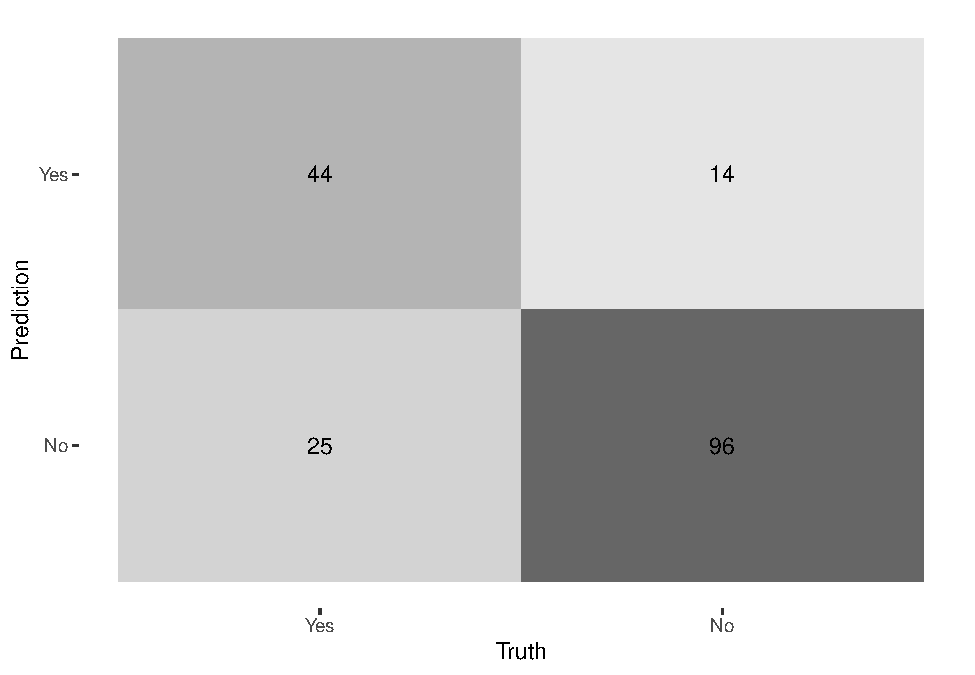
\includegraphics{hw3_files/figure-latex/unnamed-chunk-19-1.pdf}

\begin{Shaded}
\begin{Highlighting}[]
\CommentTok{\# ROC curve on the testing data}
\FunctionTok{augment}\NormalTok{(log\_fit, }\AttributeTok{new\_data =}\NormalTok{ titanic\_test) }\SpecialCharTok{\%\textgreater{}\%}
  \FunctionTok{roc\_curve}\NormalTok{(survived, .pred\_Yes) }\SpecialCharTok{\%\textgreater{}\%}
  \FunctionTok{autoplot}\NormalTok{()}
\end{Highlighting}
\end{Shaded}

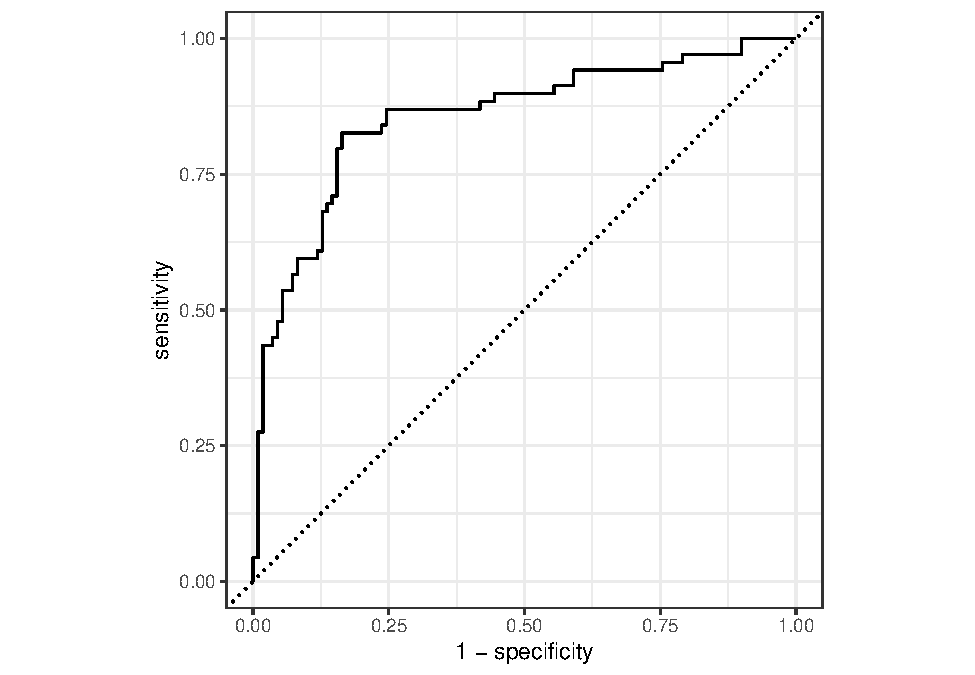
\includegraphics{hw3_files/figure-latex/unnamed-chunk-19-2.pdf}

\begin{Shaded}
\begin{Highlighting}[]
\CommentTok{\# Area under the ROC curve (AUC)}
\FunctionTok{augment}\NormalTok{(log\_fit, }\AttributeTok{new\_data =}\NormalTok{ titanic\_test) }\SpecialCharTok{\%\textgreater{}\%}
  \FunctionTok{roc\_auc}\NormalTok{(survived, .pred\_Yes)}
\end{Highlighting}
\end{Shaded}

\begin{verbatim}
## # A tibble: 1 x 3
##   .metric .estimator .estimate
##   <chr>   <chr>          <dbl>
## 1 roc_auc binary         0.856
\end{verbatim}

The training accuracy is 0.816 and the testing accuracy is 0.782. The
high accuracy indicates that the model perform well in this case. And
the higher accuracy in training dataset is reasonable because it the
model is fitted better on the traning dataset. And the AUC score looks
good. Thus the model is usable.

\end{document}
